\documentclass{standalone}
\usepackage[dvipsnames]{xcolor}
\usepackage{tikz}
\usetikzlibrary{decorations.pathmorphing,patterns}
%\usepackage{pgfplots}
%\usepackage{pgfplotstable}
%\pgfplotsset{compat=1.5}
\usetikzlibrary{patterns,decorations.markings}

\begin{document}
{
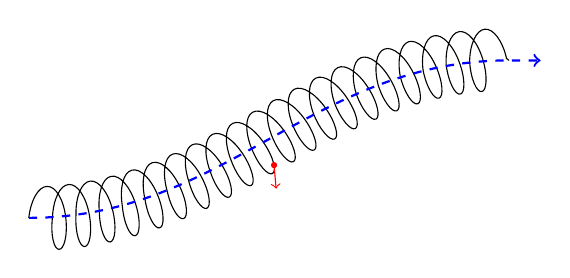
\begin{tikzpicture}
\draw[decoration={aspect=0.4, segment length=3mm, amplitude=4mm,coil},decorate] (0,5) to [out=0, in = 180] (6.1,7);
\draw[blue,->,thick,dashed] (0,5) to [out=0, in = 180] (6.1,7) -- (6.5,7);
\fill[red] (3.115,5.67) circle (0.04) node (a) {};
\draw[red,->] (a.center) -- ++(275:0.3);
\end{tikzpicture}
}
\end{document}